\section{Git Flow}\label{sec:github-flow}
\begin{frame}[c]
    \centering
    \Large
    \textbf{Git Flow}
\end{frame}

\subsection{Der Workflow}\label{subsec:der-workflow}
\begin{frame}[c]
    \slidehead
    \centering
    \large
    \textbf{Git Flow}
    \vspace{1em}
    \begin{enumerate}[<+->]
        \item \textbf{dev Branch von master abbranchen}
        \item \textbf{Kritische Hotfixes direkt auf master}
        \item \textbf{Feature Branch von dev abbranchen}
        \item \textbf{Feature implementieren}
        \item \textbf{Pull Request erstellen \& reviewen \& mergen \& löschen}
        \item \textbf{Release-Branch von dev abbranchen}
        \item \textbf{Release-Branch in master \& dev mergen}
    \end{enumerate}
\end{frame}

\begin{frame}[c]
    \centering
    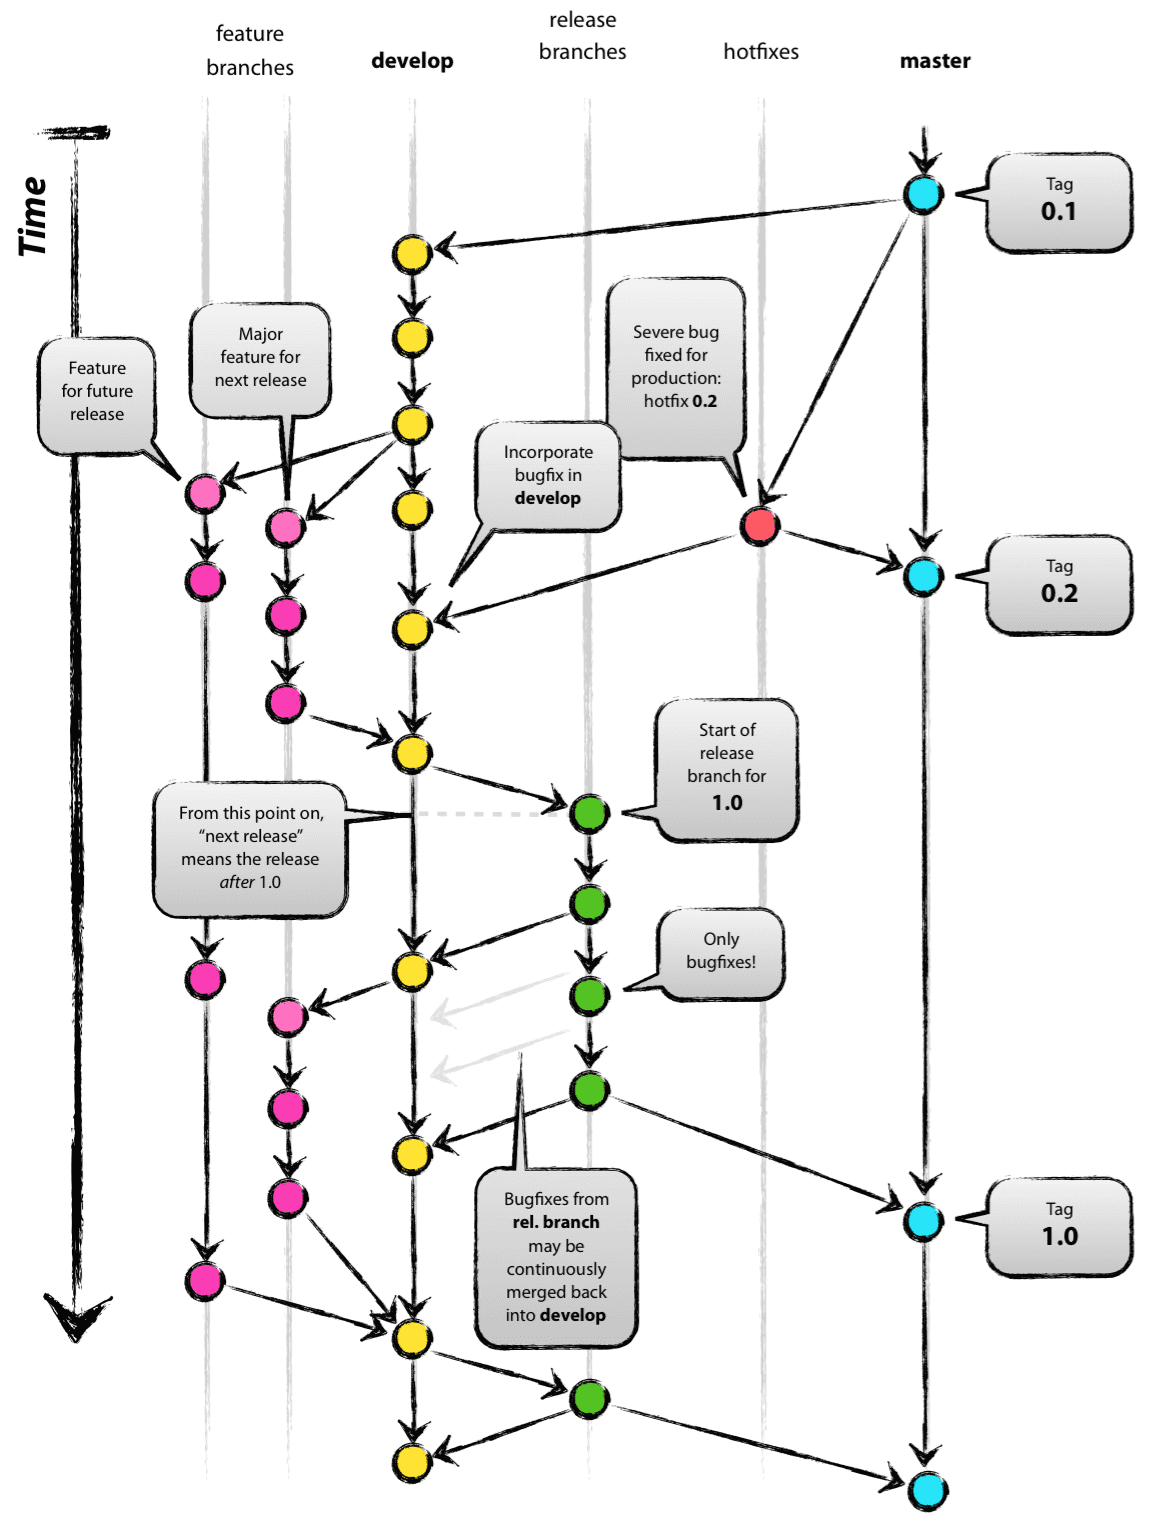
\includegraphics[scale=.15]{../../pictures/git-flow}
\end{frame}

\begin{frame}[c]
    \slidehead
    \large
    \textbf{Bewertungskriterien}
    \normalsize
    \begin{enumerate}
        \item<2-> Wie skaliert der Workflow? \only<3->{\hfill\textbf{sehr gut für große Teams}}
        \item<4-> Können Bugs/Fehler einfach in den Master-Branch gelangen? \only<5->{\hfill\textbf{ja}}
        \item<6-> Kann man Fehler einfach rückgängig machen? \only<7->{\hfill\textbf{geht}}
        \item<8-> Erzeugt dieser Workflow eine neue unnötige, kognitive Überlastung für das Team? \only<9->{\hfill\textbf{it depends}}
    \end{enumerate}
\end{frame}
